\documentclass[11pt]{beamer}
\usetheme{CambridgeUS}
\usepackage[utf8]{inputenc}
\usepackage[spanish]{babel}
\usepackage{amsmath}
\usepackage{amsfonts}
\usepackage{amssymb}
\usepackage{graphicx}
\author{Sergio Salinas}
\title{Modelamiento base de datos para tu proyecto científico}
%\setbeamercovered{transparent} 
%\setbeamertemplate{navigation symbols}{} 
%\logo{} 
%\institute{USACH} 
%\date{} 
%\subject{} 
\begin{document}

\begin{frame}
\titlepage
\end{frame}

\begin{frame}
\tableofcontents
\end{frame}

\section{El concepto Base de datos}

\begin{frame}{¿Qué es una base de datos?}
Es una herramienta para recopilar y organizar grandes cantidades de información de manera estructurada y con la menor redundancia posible.

\begin{center}
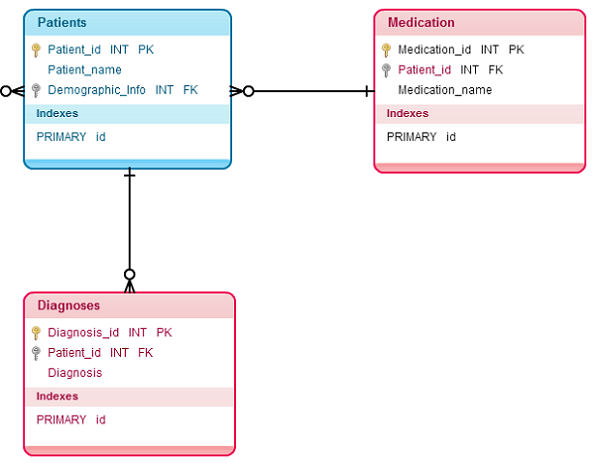
\includegraphics[scale=0.5]{images/relational-database-model1.png} 

\end{center}

\end{frame}

\begin{frame}{Base de datos dentro de un proyecto científico}

\begin{itemize}

\item  Evita la \textbf{redundancia} de datos
\item Permite hacer consultas complejas para el \textbf{análisis del contenido}
\item Permite establecer reglas a la hora de \textbf{trabajar en equipo}
\end{itemize}

\end{frame}



\begin{frame}{Ejemplo de tabla única}

\begin{table}[!ht]
\centering
\resizebox{\textwidth}{!}{
\begin{tabular}{|l|l|l|l|l|l|l|}
\hline
\multicolumn{7}{|l|}{} \\ \hline
\hline 
Nombre Paciente & Tipo   & Síntomas                      & Medico       & Rut          & E.C.    & Sueldo    \\ \hline
Sasha           & Felino & Vomito, cansancio, pelo caído & Álvaro Pérez & 16.336.789-7 & Soltero & \$500.000 \\ \hline
Luna            & Felino & Un poco vaga                  & Álvaro Pérez & 16.336.789-7 & Soltero & \$500.000 \\ \hline
Toby            & Canino & No come                       & Juan Piedra  & 15.533.559-5 & Soltero & \$700.000 \\ \hline
\end{tabular}}
\end{table}


\end{frame}


\begin{frame}{Ejemplo con más de una tabla}

\begin{table}[!ht]
\centering
\resizebox{\textwidth}{!}{
\begin{tabular}{|l|l|l|l|}
\hline
\multicolumn{4}{|l|}{Paciente} \\ \hline
\hline 
Nombre Paciente & Tipo   & Síntomas                      & Medico       \\ \hline
Sasha           & Felino & Vomito, cansancio, pelo caído & Álvaro Pérez \\ \hline
Luna            & Felino & Un poco vaga                  & Álvaro Pérez \\ \hline
Toby            & Canino & No come                       & Juan Piedra  \\ \hline
\end{tabular} 
}
\end{table}
\begin{table}[]
\centering
\resizebox{\textwidth}{!}{
\begin{tabular}{|l|l|l|l|}
\hline
\multicolumn{4}{|l|}{Medico} \\ \hline
\hline 
Nombre Paciente & Tipo   & Síntomas                      & Medico       \\ \hline
Sasha           & Felino & Vomito, cansancio, pelo caído & Álvaro Pérez \\ \hline
Luna            & Felino & Un poco vaga                  & Álvaro Pérez \\ \hline
Toby            & Canino & No come                       & Juan Piedra  \\ \hline
\end{tabular}
}
\end{table}
\end{frame}



\begin{frame}{Componentes de una Base de Datos}
\begin{itemize}

\item \textbf{Entidades} Son objetos o cosas. \textit{Persona, auto, Habitad, Paciente}

\item \textbf{Atributos} Le dan propiedades a la entidad. \textit{Persona tiene rut, nombre, peso, etc}.

\item \textbf{Identificadores} Atributo que permite diferenciar una instancia de otra en una entidad. \textit{Una persona se puede diferenciar de otra por su rut.}

\item  \textbf{Relaciones} Establecen la conexión entre dos o más entidades

\end{itemize}


\begin{center}
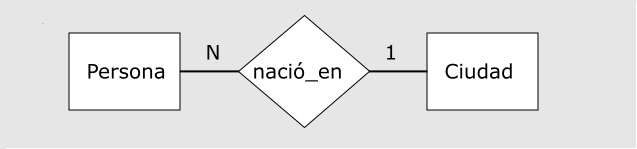
\includegraphics[scale=0.5]{images/rel.png} 
\end{center}


\end{frame}


\begin{frame}{Entidad como Una tabla}
\begin{table}[!H]
\begin{tabular}{|c|c|c|c|}
\hline
\multicolumn{4}{|l|}{Persona} \\ \hline
\hline 
Rut & Nombre & Ocupación & Peso \\ 
\hline 
15.654.896-6 & Juan & Trabajador & 70 \\ 
\hline 
23.459.786-1 & Maria & Estudiante & 60 \\ 
\hline 
\end{tabular} 
\end{table}

La entidad es Persona, sus atributos Rut, nombre, Ocupación y Peso.\\
El identificador de la entidad es el rut ya que es único.\\
Juan y María son instancias de la entidad Persona.\\

\end{frame}





%\begin{frame}{Base de datos por sobre hojas de calculo}
%\begin{center}
%
\includegraphics[scale=.5]{images/excel-worlds-most-used-database.jpg} 

%\end{center}


%\end{frame}


\section{Modelamiento}

\begin{frame}{Problema inicial}

Un equipo de investigación desea estudiar los medicamentos que los doctores les dan a sus pacientes. Para ello deciden crear una base de datos, hasta ahora estos son los datos que desean almacenar.

\begin{itemize}



\item Para cada paciente se desea almacenar su rut, nombre y su diagnostico.

\item Para cada medicamento guardar su Identificador único, nombre y componente activo.

\item Para cada doctor, registrar su rut, nombre y área en la que se desempeña.

\end{itemize}

Tomar en cuenta que cada paciente tiene un solo medico y un paciente puede tomar varios medicamentos a la vez.

\end{frame}

\end{document}